\subsection{Model Reduction}

Before we can design a controller to stabilize the roll and pitch motion of the robot, we must first understand the dynamics of the system. Previous works, \cite{glasheen1996hydrodynamic}, \cite{floyd2008design}, \cite{hsieh2004running}, have considered the coupled vertical and horizontal kinematics and dynamics of the basilisk lizard. These works found that the Basilisk Lizard produces lift and thrust by cycling its feet through the water surface in three distinct phases: slap, stroke, and recovery. In the slap and stroke phases, the lizard generates vertical and horizontal forces primarily via fluid drag on the foot. Then during the retraction phase, the lizard withdraws its foot within the lingering air cavity produced by the high velocity of the foot during the slap phase, thereby greatly reducing downwards drag forces during this phase. 

The above studies provide detailed and comlex descriptions of generated forces and dynamics during water surface locomotion. Specifically, complexity in these models arise from the hybrid dynamics impsosed by the water contact discontinuity, the nonlinearity of drag forces and the curse of dimensionality. For the purposes of controller design, the complexity of previously developed models for water surface locomotion may limit intuition, provide more information than is necessary to accomplish the desired task, and preclude the development of analytical expressions for generated force and robot state. Therefore, to simplify and focus our analysis on the dynamics required to understand pitch and roll motions, we will only consider vertical dynamics produced by a simplified foot trajectory in the following analysis. 

Figure~\ref{fig:trajrob} shows the foot trajectory  and the corresponding phase diagram of the previously built water runner robot \cite{park2010roll}. In contrast, figure~\ref{fig:trajsimp} shows a simplified circular foot trajectory and its corresponding phase diagram. We can see from the phase diagrams of the two trajectories that, especially during the plunge and stroke stages, the $y$-kinematics of the simplified foot trajectory and the actual foot trajectory are quite similar. This suggests that the $y$-dynamics produced by these two trajectories may also be similar.

\begin{figure}[tb]
	\centering
	\begin{subfigure}[t]{0.48\textwidth}
		\centering
		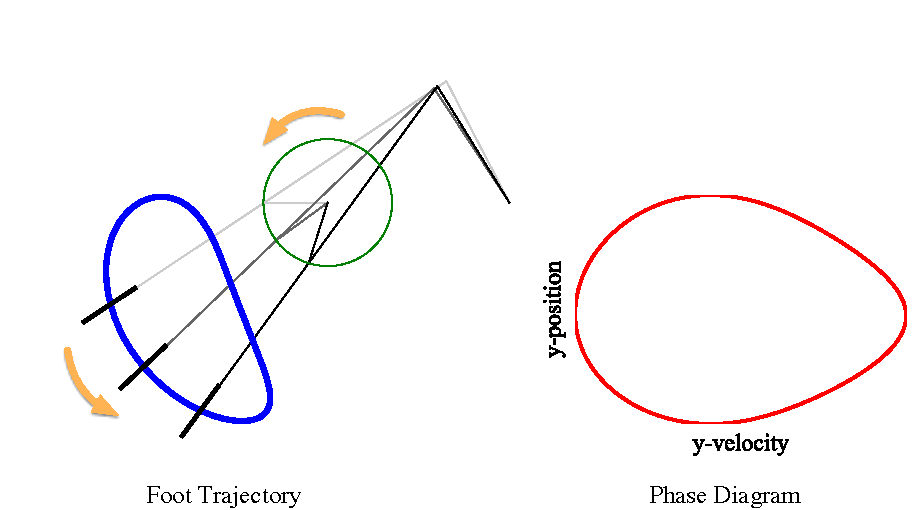
\includegraphics[width = \textwidth]{figures/foot_trajs.pdf}
		\caption{The water runner robot's foot locus in blue, with three instantaneous configurations of the leg's four-bar mechanism shown in grey. The circular path traced by the joint at the end of the input link is traced in green. In red is the phase diagram of this legged system.}
		\label{fig:trajrob}
	\end{subfigure}

	\begin{subfigure}[t]{0.48\textwidth}
		\centering
		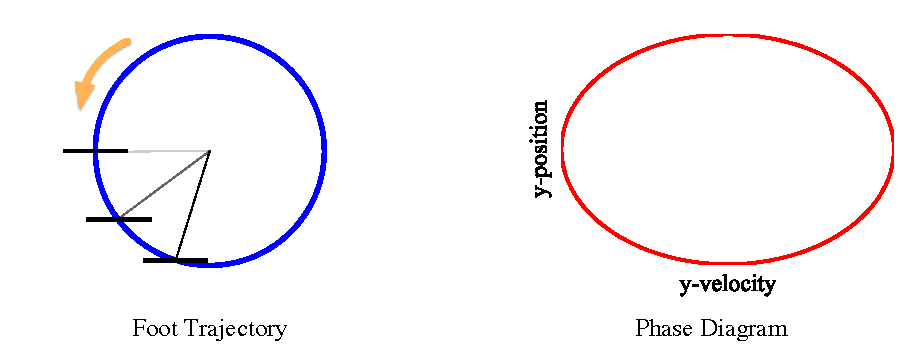
\includegraphics[width = \textwidth]{figures/foot_trajs2.pdf}
		\caption{A simplified circular foot locus in blue, with three instantaneous leg configurations shown in grey. In red is the phase diagram of this model.}
		\label{fig:trajsimp}
	\end{subfigure}
	\caption{Trajectories and phase portraits for the water runner robot and a simplified model. Note that the orientation of the foot pad of the actual robot follows the orientation of the leg, whereas the orientation of the foot pad in the simplified mode is constant.}
	\label{fig:traj}
\end{figure}

\subsection{Force Generation}
Because we are neglecting the horizontal kinematics of the system, the simplified circular foot trajectory can be further simplified to a foot mounted on a prismatic joint traveling vertically. We can calculate the force generated by a foot traveling on this trajectory via the equation obtained by Galsheen and McMahon \cite{glasheen1996vertical}, which states that the time-varying forces exerted by water during vertical impact of disks follows,

\begin{equation}
	F(t) = - C_D^* \left[\frac{1}{2} S \rho \dot{y}(t) |\dot{y}(t) | + S \rho g y(t) \right]
	\label{eq:force_t}
\end{equation}

\noindent where $F(t)$ is the time varying drag force, $C_D^* \approx 0.703$ is the drag coefficient, $\rho$ is the density of water, $g$ is the acceleration due to gravity, $S$ is the effective circular area of the disk, and $y(t)$ and $\dot{y}(t)$ are the time-varying vertical position and velocity of the disk measured in a coordinate system where positive $y$ opposes the gravity vector. 

Equation~\ref{eq:force_t} shows that the magnitude of the force force has a quadratic dependence on foot pad speed, as one would expect given the high-Reynolds number regime in which the foot operates. Therefore, the robot should generate significantly more lift by plunging its foot into the water faster than it retracts its foot.

We now introduce a new parameter, duty factor $(DF)$, which is the ratio of the time the foot spends traveling downwards over the total time of one cycle. With this definition, we can find the angular velocity during the downwards half of the trajectory $\omega_1$ and the angular velocity during the upwards half of the trajectory $\omega_2$, given an average angular velocity $\omega$.

\begin{align}
	\omega_1 &= \frac{\omega}{2 DF} \\
	\omega_2 &= \frac{\omega}{2 (1 - DF)} 
\end{align}

With duty factor incorporated into equation 1, we can write the vertical dynamics of a one legged system as in figure~\ref{fig:trajsimp} as the following system of differential equations:

\begin{equation}
	\frac{d}{dt} \begin{bmatrix} y(t) \\ \dot{y}(t) \end{bmatrix} = \begin{bmatrix} \dot{y}(t) \\ F(y(t),\dot{y}(t), DF(t)) \end{bmatrix} - \begin{bmatrix} 0 \\ mg \end{bmatrix}
	\label{eq:eom}
\end{equation}

In order to solve for the dynamics of the system we must reduce some of the complexity outlined earlier, First we can deal with the curse of dimensionality by assuming that the velocity of the robot body oscillations are much less than the velocity foot oscillations. This assumption is justified given the high operational frequency range of the robot (7 - 12 Hz), the quadratic damping of the water, and the relative masses of the robot body and the footpad.
	
Next to deal with the hybrid nature of the system, we will look at the average force generated in one cycle. This assumption transforms the continuous system represented by \ref{eq:eom} into a discrete-time system following the update rule:

\begin{equation}
	\begin{bmatrix} y_{t+1} \\ \dot{y}_{t+1} \end{bmatrix} = \begin{bmatrix} y_{t} \\ \dot{y}_{t} \end{bmatrix} + \left( \begin{bmatrix}  \dot{y}_t \\ F_{avg}(y_t,\dot{y}_t, DF_t) \end{bmatrix} - \begin{bmatrix} 0 \\ mg  \end{bmatrix} \right) \frac{2 \pi}{\omega}
	\label{eq:eom_discrete}
\end{equation}

We can now develop an expression for $F_{avg}$ given $y_t$, $\dot{y}_t$, and $DF_t$. First we define several constants. The drag coefficient of the water impact force is $b = \frac{1}{2} C_d S \rho$, the stiffness coefficient of the water impact force is $C_d S \rho g$, the height of the center of the foot trajectory with respect to the water is $h$, the amplitude of the foot oscillation is $A$, and the reduction in forces during the upwards part of the trajectory due to the air cavity and folding foot designs is $\alpha$. Given the zero-body motion assumption we have made we can express the position and velocity of the foot as

\begin{align}
	y &= A \cos(\omega_i t) + h \\
	\dot{y} &= -A \omega_i \sin (\omega t)
\end{align}

\noindent Where $i \in \{1,2\}$. The average force on the foot is given by 

\begin{align}
	F_{avg} &= \frac{\omega}{2 \pi} \int_0^{\frac{2 \pi}{\omega}} (-b \dot{y} | \dot{y} | - k y) dt \notag \\
			&= \frac{\omega}{2 \pi} \int_{t_1}^{\frac{\pi}{\omega_1}} \left[ b A^2 \omega_1^2 \sin^2 \omega_1 t - k A \cos \omega_1 t - kh  \right] dt \notag \\
			&\quad + \frac{ \alpha \omega}{2 \pi}  \int_{\frac{\pi}{\omega_2}}^{t_2} \left[ -b A^2 \omega_2^2 \sin^2 \omega_2 t - k A \cos \omega_2 t - kh \right] dt \label{eq:eom_int}
\end{align}

\noindent Where $t_1$ is the time of contact with the water surface and $t_2$ is the time of exit from the water surface given by 

\begin{align}
	t_1 &= \frac{2 DF}{\omega} \left( \pi - \arccos \frac{h}{A} \right) \\
	t_2 &= \frac{2 (1 - DF)}{\omega} \left( \pi + \arccos \frac{h}{A}\right)
\end{align}

\noindent Evaluating equation~\ref{eq:eom_int} with the above limits gives

\begin{align}
	F_{avg} &= \frac{b A^2 \omega^2}{8 \pi} \left( \arccos \left(\frac{h}{A}\right) - \frac{h \sqrt{A^2 - h^2}}{A^2} \right) \notag \\
		    &\quad \times \left( \frac{1}{DF} - \frac{\alpha}{1 - DF} \right) \notag \\
			&\quad + \frac{k}{\pi}  \left( \sqrt{A^2 - h^2} - h \arccos \left(\frac{h}{A}\right) \right) \notag \\
			&\quad \times (DF + \alpha (1-DF)) \label{eq:eom_avg}
\end{align}

\subsection{Model Fitting}

To ensure the above model represents the actual system as well as possible, we fit the model to the data using two parameters via non-linear least squares regression. The first is $S$, the 
effective area of the foot pad and the second is $A$ the amplitude of the foot oscillation. The need to fit these two parameters arise from the time-dependent angle of the footpad of the real robot, which the simplified model does not capture. The angle of the foot pad requires we use an average projected area onto the $xz$-plane, as this is the area component that produces forces in the $y$-direction. Also, the angle of the foot pad reduces the effective amplitude of the foot trajectory because the angled foot pad enters the water gradually. Thus the force generated during the slap phase increases gradually, and not instantly as in the simple model predicts.

To obtain the data to fit our model to, we record the average limit-cycle heights of the simulated robot for foot cycle frequencies from 20 to 100 rad/s. Then we solve for the steady state height solve for the steady state height as predicted by equation~\ref{eq:eom_avg}. I.e. solve for $h$ such that $F_{avg} - mg = 0$.

The area $S$ that results from the least-squares fitting represents an average projected area on to the $x-y$ plane while 

